\documentclass[10pt]{beamer}
\definecolor{title}{RGB}{1, 45, 112}
\definecolor{body}{RGB}{218, 233, 255}
\definecolor{background}{RGB}{250, 250, 250}
\usetheme[progressbar=frametitle]{metropolis}
\usecolortheme{wolverine}
\usefonttheme{professionalfonts}
\setbeamertemplate{navigation symbols}{}
\setbeamercolor{block title}{bg=title,fg=white}
\setbeamercolor{block body}{bg=body!40,fg=black}
\setbeamertemplate{section in toc}[square]
\setbeamertemplate{subsection in toc}[square]

\usepackage{graphicx}
\graphicspath{ {../images/} }

\usepackage{tikz}
\tikzset{
    use page relative coordinates/.style={
        shift={(current page.south west)},
        x={(current page.south east)},
        y={(current page.north west)}
    },
}

\usepackage{algpseudocode}

\usepackage[T1]{fontenc}
\usepackage{libertinus}
\usepackage{listings}

% settings for code listings (colors and appearence)
\definecolor{codegreen}{rgb}{0,0.6,0}
\definecolor{codegray}{rgb}{0.5,0.5,0.5}
\definecolor{codepurple}{rgb}{0.58,0,0.82}
\definecolor{backcolour}{rgb}{0.95,0.95,0.92}

\lstdefinestyle{mystyle}{
    backgroundcolor=\color{backcolour},   
    commentstyle=\color{codegreen},
    keywordstyle=\color{blue},
    numberstyle=\tiny\color{codegray},
    stringstyle=\color{codepurple},
    basicstyle=\ttfamily\footnotesize,
    breakatwhitespace=false,         
    breaklines=true,                 
    captionpos=b,                    
    keepspaces=true,                 
    numbers=left,                    
    numbersep=5pt,                  
    showspaces=false,                
    showstringspaces=false,
    showtabs=false,                  
    tabsize=2
}

\lstset{style=mystyle}

\usepackage{bm}
\usepackage{amsmath, amssymb}
\DeclareMathOperator{\sign}{sign}
\DeclareMathOperator{\rank}{rank}
\DeclareMathOperator{\energy}{E}

\usepackage{ragged2e}
\justifying

\usepackage[backend=biber, style=ieee]{biblatex}
\addbibresource{references.bib}
\nocite{*}

\title{Singular Value Decomposition}
\subtitle{An application to Big Data}
\author{Davide Sferrazza}
\institute{Università degli Studi di Palermo}
\date{\today}

\def\titlepage{%
  \usebeamertemplate{title page}%
}

\begin{document}
\maketitle

\begin{frame}
    \frametitle{Outline}
    \tableofcontents
\end{frame}

\section{Singular Value Decomposition}
\subsection{What is it?}

\begin{frame}
    \frametitle{Definition of SVD}
    \begin{theorem}
        Given a matrix $A \in \mathbb{R}^{m \times n}$, it can always be found a decomposition such that
        \begin{equation}
            \label{eq:SVD}
            A = U \Sigma V^T
        \end{equation}
        where $U \in \mathbb{R}^{m \times m}$, $V \in \mathbb{R}^{n \times n}$ and $\Sigma \in \mathbb{R}^{m \times n}$.

        $U$ and $V$ are two orthogonal matrices and $\Sigma$ is a diagonal matrix, namely:
        $$ ( \Sigma )_{ij} = 
            \begin{cases}
                \sigma_i, & i = j \\
                0, & i \ne j 
            \end{cases} 
        $$
        where $\sigma_1 \ge \sigma_2 \ge \ldots  \ge \sigma_p \ge 0$, $p = \min\{m, n\}$.
    \end{theorem}
\end{frame}

\begin{frame}
    \frametitle{Definition of SVD}
    The non-zero entries of $\Sigma$, denoted by $\sigma_i$, are called \textit{singular values}.

    They are arrenged in a nonincreasing order by convention.

    The column vectors $\bm{u_i}$ of $U$ are called \textit{left singular vectors} and those $\bm{v_i}$ of $V$ are called \textit{right singular vectors}. \bigskip
    
    Since in general $m \ne n$, we have: 
    $$ A = \sum_{i = 1}^{p} \bm{u_i} \sigma_i \bm{v_i}^T $$

\end{frame}

\begin{frame}{Definition of SVD}
    \begin{theorem}
        If for some $r$ such that $ 1 \le r < p $ we have
        $$ \sigma_1 \ge \ldots \ge \sigma_{r} > \sigma_{r + 1} = \ldots = \sigma_p = 0  $$
        then
        \begin{itemize}
            \item $\rank(A) = r$
            \item $ A = \sum \limits_{i = 1}^{r} \bm{u_i} \sigma_i \bm{v_i}^T $
        \end{itemize}
    \end{theorem}

    It means that all other $p-r$ dimensions of matrix $A$ are linear combinations of the first $r$.
\end{frame}

\begin{frame}{Definition of SVD}
    \begin{block}{Lower rank approximation}
        Let $A \in \mathbb{R}^{m \times n}$ be a matrix whose rank is $\rank(A) = r$. \\
        If for a fixed integer value $k < r$ we define
        \begin{equation}
            \label{eq:lower_rank}
            A_k = \sum \limits_{i = 1}^{k} \sigma_i \bm{u_i}  \bm{v_i}^T 
        \end{equation}
        and
        $$ \mathcal{B} = \left\{ B \in \mathbb{R}^{m \times n} : \rank(B) = k \right\}$$
        then 
        $$ \min_{B \in \mathcal{B}} \left\lVert A - B \right\rVert _2 = \left\lVert A - A_k \right\rVert _2 = \sigma_{k + 1} $$
    \end{block}
        
    This result tell us that $A_k$ represents the best approximation (considering the \textit{spectral norm}) of rank $k$ of matrix $A$.
\end{frame}

\subsection{How can singular values be computed?}

\begin{frame}{Singular values computation}
    To compute the singular values, consider the transponse of $A$ given its decomposition:
    $$ A^T = (U \Sigma V^T)^T = V \Sigma^T U^T$$
    The symmetric matrix $A^T A$ is equal to:
    $$ A^T A = ( V \Sigma^T U^T )(U \Sigma V^T) = V \Sigma^T \Sigma V^T$$
    Furthermore, this equation can be written as:
    $$ A^T A V = V \Sigma^T \Sigma $$
    It means that the diagonal entries of the square matrix $ \Sigma^T \Sigma $, which are the square of the singular values, are the eigenvalues of matrix $A^T A$ and $ V $ is the matrix of eigenvectors.
\end{frame}

\begin{frame}{Singular values computation}
    Similarly, consider the product of $A A^T$. It is equal to:
    $$ A A^T = (U \Sigma V^T)( V \Sigma^T U^T ) = U \Sigma \Sigma^T U^T$$
    Which means that:
    $$ AA^T U = U \Sigma \Sigma^T $$
    Hence $U$ is the matrix of eigenvectors of $AA^T$. \bigskip

    Since $\rank(A) = r$, only the first $r$ eigenvalues of $AA^T$ and $A^T A$ are non-zero.
\end{frame}

\section{Finding eigenvalues and eigenvectors}
\subsection{QR Method}

\begin{frame}{QR Method}
    A possible method to find eigenvalues and eigenvectors of a matrix is based on $QR$ decompositions and this theorem:
    \begin{theorem}
        Suppose $A \in \mathbb{R}^{n \times n}$ is a matrix having eigenvalues $\lambda_1, \lambda_2, \ldots \lambda_n$ satisfying 
        \begin{equation}
            \label{eq:eigenvalues_rel}
            \left\lvert \lambda_1 \right\rvert > \left\lvert \lambda_2 \right\rvert > \ldots > \left\lvert \lambda_n \right\rvert
        \end{equation}
        then the following sequence for $A_1 = A$ and $k = 1, 2, \ldots$
        \begin{equation}
            \label{eq:A_sequence}
            \begin{cases}
                A_k = Q_k R_k \\
                A_{k+1} = R_k Q_k 
            \end{cases} 
        \end{equation}
        converges to an upper triangular matrix where $(A_k)_{ii} = \lambda_i, \, i = 1, 2, \ldots, n$.
        In case (\ref{eq:eigenvalues_rel}) is not satisfied, this sequence converges to a triangular matrix with square blocks of order at most 2 along the diagonal. \newline
        If $A$ is symmetric, then the sequence converges to a diagonal matrix. 
    \end{theorem}
\end{frame}

\begin{frame}[fragile]{QR Method}
    So a basic implementation would be like this:
    \begin{lstlisting}[language=Matlab]
    while err > toll
        [Q, R] = qr(A);
        A = R * Q;

        err = max( max( abs( tril(A, -1) ) ) );
    end \end{lstlisting}
    This method can be sped up by using a technique called \textit{shifting}:
    \begin{lstlisting}[language=Matlab]
    n = length( A );
    while err > toll
        % A(n, n) is a usual choice, it can be any real number
        T = A(n, n) * eye(n);
        [Q, R] = qr( A - T );
        A = R * Q + T;

        err = max( max( abs( tril(A, -1) ) ) );
    end \end{lstlisting}
\end{frame}

\begin{frame}{QR Method}
    In our case, this method must be applied to $A A^T$ and $A^T A$, so if (\ref{eq:A_sequence}) converges then we have a diagonal matrix. \newline
    Now, consider the diagonalization of $B$, where $B = A A^T$ or $B = A^T A$:
    $$
    B = P \Lambda P^{-1} =  P \Lambda P^T
    $$
    As $B$ can be factored using (\ref{eq:A_sequence}), the matrix containing the eigenvectors must be equal to:
    $$
    P = \prod_i Q_i = Q_1 Q_2 Q_3 \cdots
    $$ \bigskip

    Hence, for every iteration $B_k = Q_k R_k$ and $B_{k+1} = R_k Q_k$, requiring each step to have a computational cost equal to $O(\frac{2 n^3}{3})$.
\end{frame}

\subsection{Improving QR Method using Givens rotation matrices}

\begin{frame}{Hessemberg Reduction}
    To achieve a lower computational cost, one solution consists in transforming $B$ in a similar tridiagonal matrix using Householder matrices. \newline
    A triangular matrix can be obtained because $B$ is symmetric. \\  \bigskip
    In general, the process of trasforming a matrix in a similar matrix using Householder matrices allows us to obtain a matrix in which $B_{ij} = 0$, for all $i > j + 1$. Such a matrix is called a \textit{Hessemberg matrix}. \bigskip

    Consequently, after $B$ has been transformed, each step of the previous code can be realized using \textit{Givens rotation matrices}.
\end{frame}

\begin{frame}{Givens rotation matrices}
    A \textit{Givens rotation} can be represented with the following matrix:
    $$
    G_{ij} =
    \begin{pmatrix}
        1 & \cdots & 0 & \cdots & 0 & \cdots & 0 \\
        \vdots & \ddots & \vdots & & \vdots & & \vdots \\
        0 & \cdots & c & \cdots & -s & \cdots & 0 \\
        \vdots & & \vdots & \ddots & \vdots & & \vdots \\
        0 & \cdots & s & \cdots & c & \cdots & 0 \\
        \vdots & & \vdots & & \vdots & \ddots & \vdots \\
        0 & \cdots & 0 & \cdots & 0 & \cdots & 1
    \end{pmatrix}
    $$ \\ \bigskip \bigskip

    where $c = \cos \theta$ and  $s = \sin \theta$, for a particular value of $ \theta \in [0, \, 2 \pi] $. \newline
    A rotation occurs in the plane spanned by the two coordinates axes $i$ and $j$.

    \begin{tikzpicture}[remember picture,overlay,use page relative coordinates]
        \node (a) at (0.75,0.636) {};
        \draw[stealth-] (a) --++ (0.07,0.0) node[circle,fill=background,at end] {i};
        \node (b) at (0.75,0.516) {};
        \draw[stealth-] (b) --++ (0.07,0.0) node[circle,fill=background,at end] {j};
        \node (c) at (0.477,0.38) {};
        \draw[stealth-] (c) --++ (0.0,-0.1) node[circle,fill=background,at end] {i};
        \node (d) at (0.592,0.38) {};
        \draw[stealth-] (d) --++ (0.0,-0.1) node[circle,fill=background,at end] {j};
    \end{tikzpicture}
\end{frame}

\begin{frame}{Givens rotation matrices}
    Using the following values:
    $$
    \begin{aligned}
        \cos \theta &=  \cfrac{\left\lvert b_{ii} \right\rvert}{ \sqrt{ b_{ii}^2 +   b_{ji}^2} } \\
        \sin \theta &= \sign \left( \cfrac{ b_{ji} }{ b_{ii} } \right)   \, \cfrac{\left\lvert b_{ji} \right\rvert}{ \sqrt{ b_{ii}^2 +   b_{ji}^2} } \\
    \end{aligned}
    $$
    when $B$ gets left multiplied by $G_{ij}$, the final matrix will have the element in position $(j, \, i)$\footnote{Note that the indices are reversed} equal to $0$. \newline
    Therefore, instead of factoring $B$ at each step by the $QR$ method, if $B$ is tridiagonal, we can simply iterate $n - 1$ times by constructing $G_{k\,k+1}$ and eliminating the elements in position $(k+1, \, k)$ and $(k, \, k+1)$.
\end{frame}

\begin{frame}{Pseudocode for finding eigenvalues and eigenvectors}
    A pseudocode of what to do should clarify what we have done so far (excluding shifting for brevity):
    \begin{algorithmic}
        \footnotesize
        \State $B, P \gets $ hessemberg($ B $)
        \While{error > toll}
            \For{$k = 1, 2, \ldots, n$}
                \State construct $G_{k \, k+1}$
                \State $B \gets G_{k \, k+1} B$
            \EndFor
            \For{$k = 1, 2, \ldots, n$}
                \State $B \gets B G_{k \, k+1}^T$
                \State $P \gets P G_{k \, k+1}^T$
            \EndFor
            \State update error
        \EndWhile
    \end{algorithmic}
    The function implementing the Hessemberg reduction must also return the matrix used for the transformation, meaning that $B = P H P^T$. \newline
    Note that $P$ is updated in this way because $Q_i = G_{12}^{(i)} G_{23}^{(i)} \cdots G_{n-1 \, n}^{(i)}$, where $i$ denotes the generic iteration for error minimization.
\end{frame}

\section{The Algorithm}

\subsection{Calculate U given V}

\begin{frame}{Calculation of left singular vectors}
    Suppose we start computing $V$ by the method explained in the previous slides. \newline
    We apply the method to $A^T A$ and get $P = V$ and $B = \Sigma^2$. \newline
    Once we have take the square root of the singular values, by explicitly writing $\Sigma$, the matrix containing the left singular vectors can be calculated as:
    $$
    A = U \Sigma V^T \Rightarrow U = A V \Sigma^{-1}
    $$
    Unlike (\ref{eq:SVD}), $U$ is a rectangular matrix, and $\Sigma$ and $V$ are square matrices. \newline
    The algorithm is now complete. The next slides will illustrate the code.
\end{frame}

\subsection{Code}

\begin{frame}[fragile]{Function to calculate Givens rotation matrices}
    \lstinputlisting[language=Matlab]{../givens.m}
\end{frame}

\begin{frame}[fragile, allowframebreaks]{Function to calculate the Hessemberg reduction}
    \lstinputlisting[language=Matlab]{../hessemberg.m}
\end{frame}

\begin{frame}[fragile, allowframebreaks]{Function to calculate singular values and singular vectors}
    \lstinputlisting[language=Matlab]{../singular_vectors.m}
\end{frame}

\begin{frame}[fragile, allowframebreaks]{Function to calculate SVD}
    \lstinputlisting[language=Matlab]{../custom_svd.m}
\end{frame}

\section{Application to Big Data}

\subsection{Dimensionality reduction}

\begin{frame}{Dimensionality reduction}
    The SVD decomposition can be applied to Big Data in order to reduce the dimensionality of data sets. \\ \bigskip

    As an example, consider the data set \cite{10.1007/978-3-030-35249-3_76} containing $33$ different attributes for $145$ students, which includes student ID, personal information and data, and higher education performance ratings\footnote{\url{https://archive.ics.uci.edu/ml/datasets/Higher+Education+Students+Performance+Evaluation+Dataset}}. \\
    Dimensionality can be reduced as follows:
    \begin{enumerate}
        \item truncate the SVD retaining top-$k$ singular values, $A \approx U_k \Sigma_k V_k^T$;
        \item compute the modified data set as $D' = D V_k = U_k \Sigma_k$.
    \end{enumerate}
\end{frame}

\begin{frame}{Dimensionality reduction}
    $D'$ represents a new data set that corresponds to the projection of the data set $D$ on a $k$-dimensional basis system of right singular vectors. 

    \begin{block}{Number of singular values}
        As indicated in \cite{leskovec2020mining}, a usual choice of $k$ is dictated by maintaining enough singular values to make up $90 \% $ of the energy in $\Sigma$. \\
        The total energy of a data set is:
        $$ \energy ( \Sigma )  = \sum_{i = 1}^{r} \sigma_i^2 $$
        where $r = \rank (D)$.
    \end{block}

    By plotting the singular values we can get an insight of how they are distributed and how many of them we can retain. 
\end{frame}

\begin{frame}{Magnitudes of singular values}
    \begin{figure}[t]
        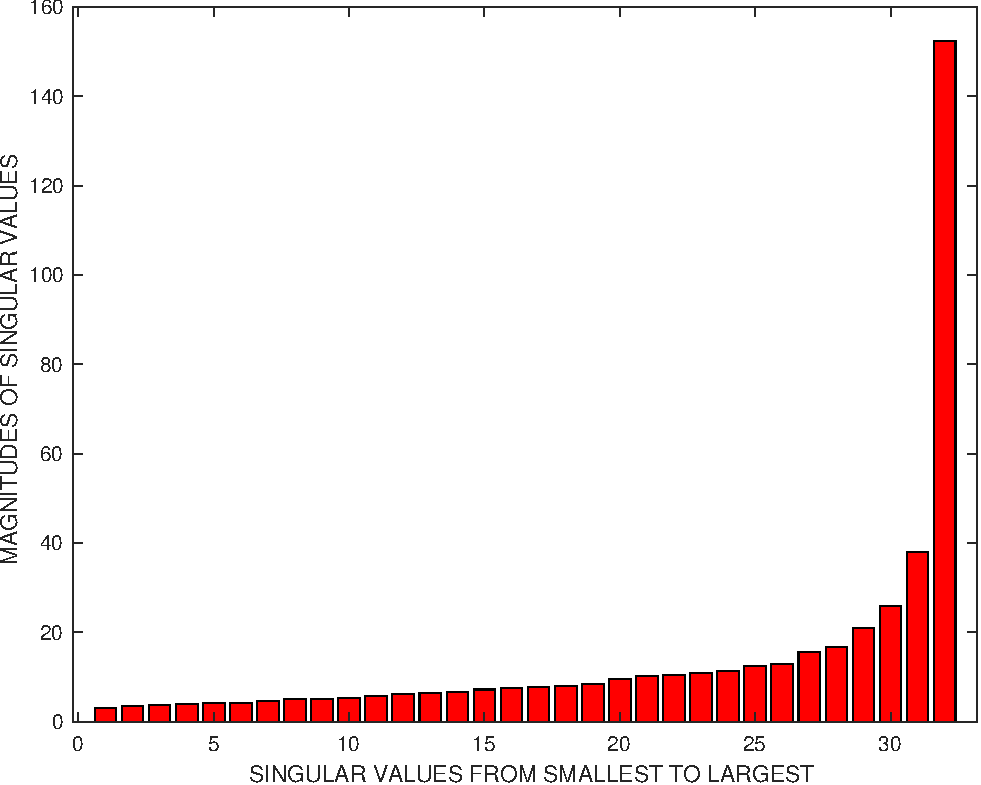
\includegraphics[width=9cm]{singular_values_magnitudes.pdf}
        \centering
    \end{figure}
\end{frame}

\begin{frame}{Retained energy}
    From what we can see, with $3$ singular values we can get about $25,346$ of energy, which is enough to exceed $90 \%$ of $\energy ( \Sigma ) = 27,830$. 
    \begin{figure}[t]
        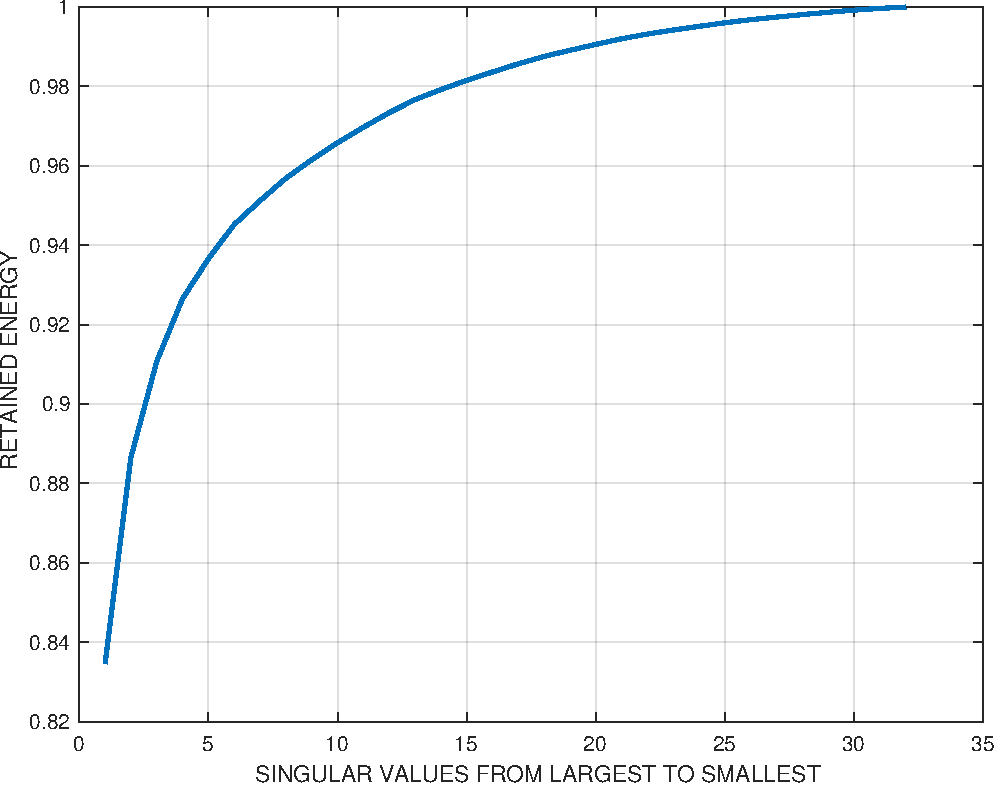
\includegraphics[width=7.7cm]{retained_energy.pdf}
        \centering
    \end{figure}
\end{frame}

\begin{frame}{Decreasing error as singular values increase}
    By increasing the number of retained singular values, the following graph is obtained:
    \begin{figure}[t]
        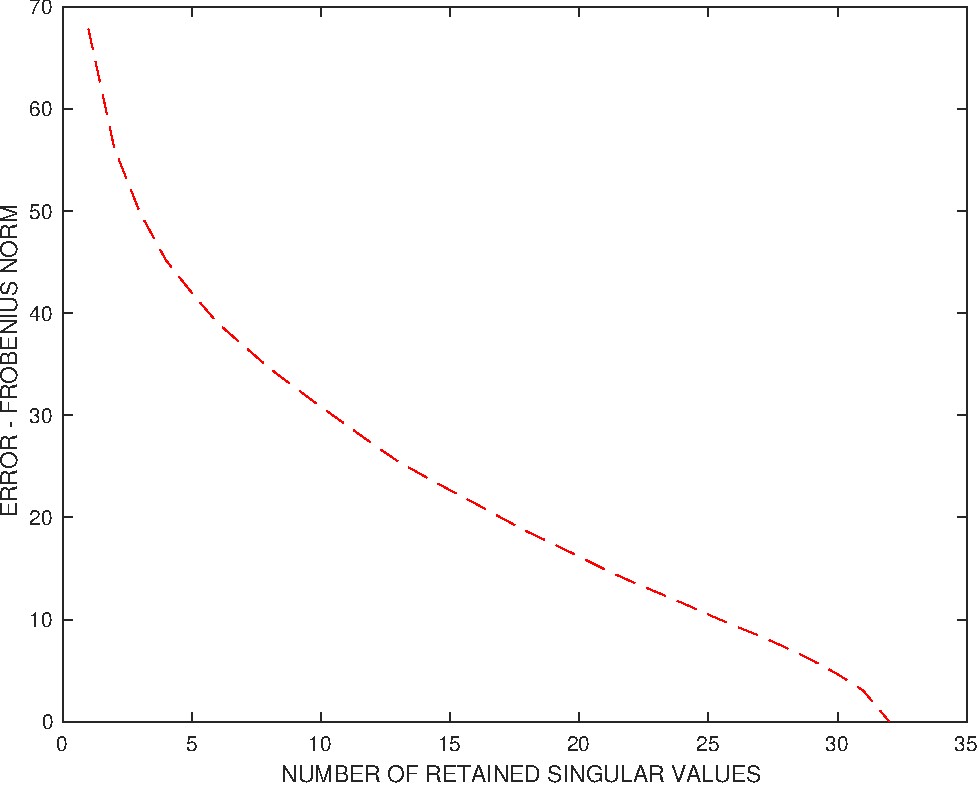
\includegraphics[width=7.7cm]{error_wrt_A.pdf}
        \centering
    \end{figure}
\end{frame}

\section{References}
\begin{frame}[plain, allowframebreaks, noframenumbering]{References}
    \printbibliography
\end{frame}

\begin{frame}{Quote}
    \begin{quote}
        \hfill "No problem can withstand the assault of sustained thinking."
    \end{quote}
    \hfill -- Voltaire
\end{frame}
\end{document}